\chapter{Ancillary Representation Analyses Figures}

\section{RNN Architecture Learned Representations}
\label{rnn_architecture_representations}

\section{MLP Architecture Learned Representations}
\label{mlp_architecture_representations}

\section{RNN Architecture with environmental and game events covariates learned representations}
\label{rnn_env_even_architecture_representations}

\section{Partitions behavioural metrics representations}
\label{partitions_behavioural}

\begin{figure}[ht]
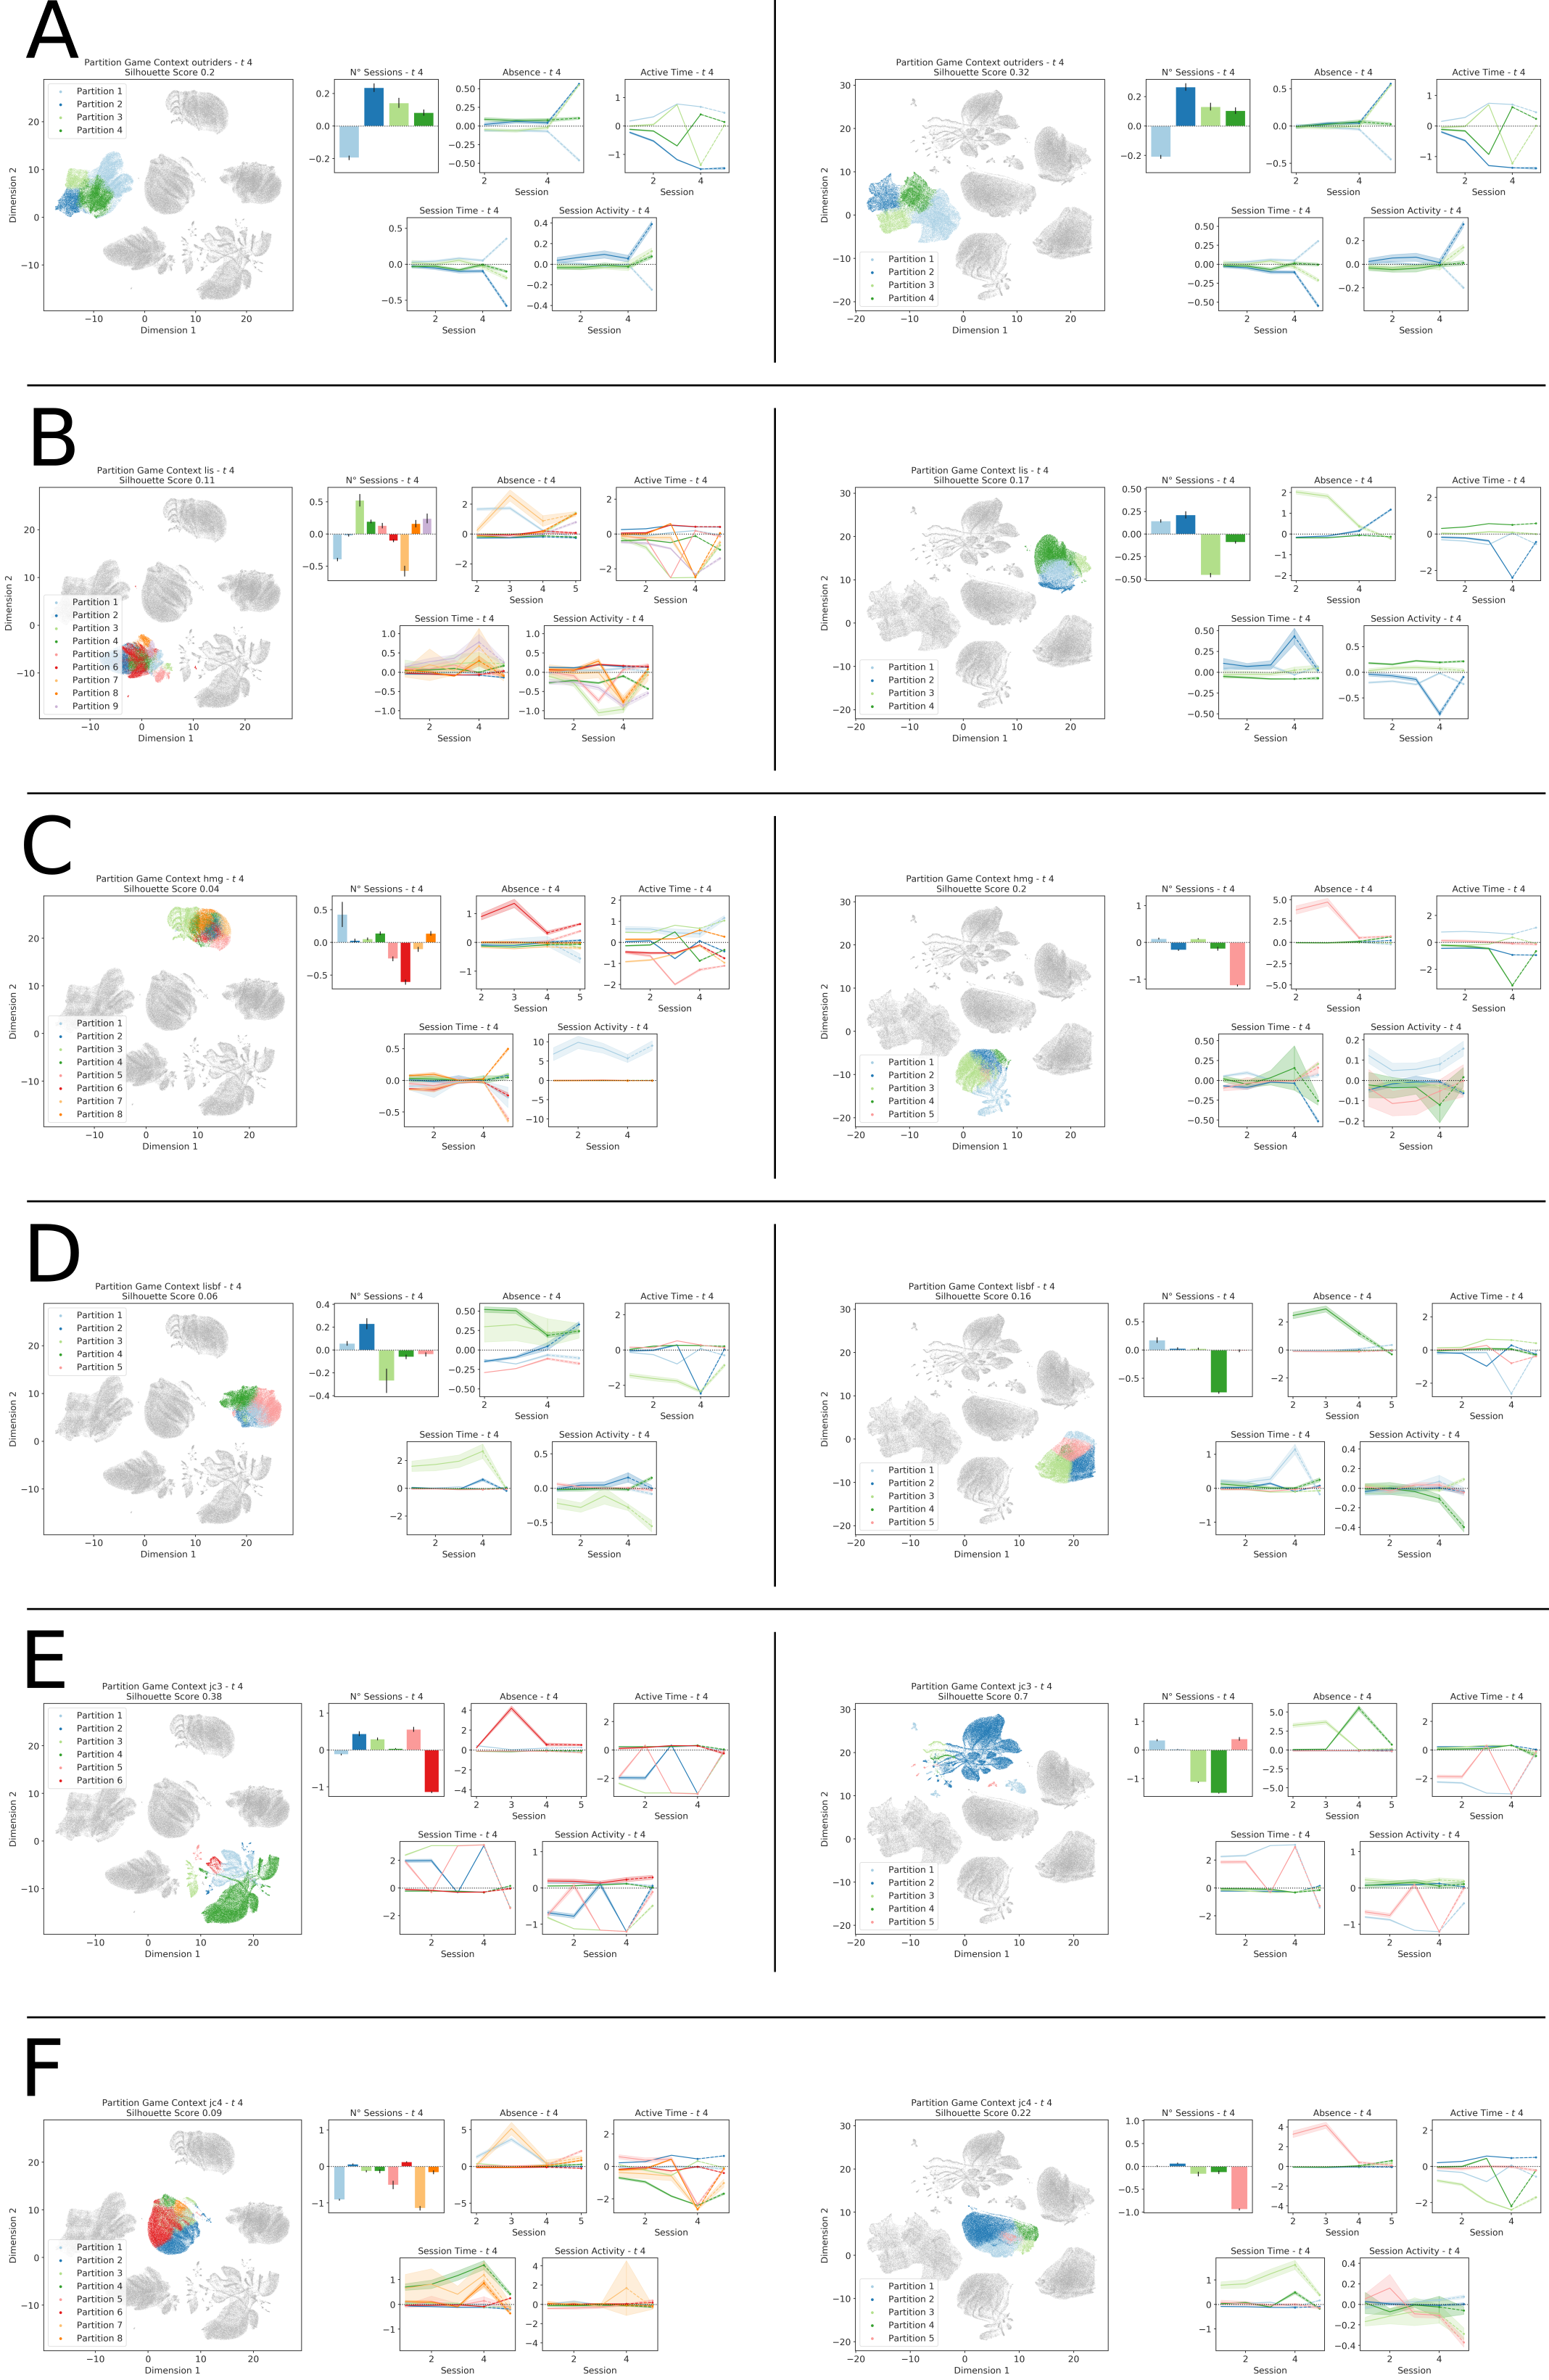
\includegraphics[width=0.7\textwidth]{images/appendix_D/clust_beha_all.png}
\centering
\caption[Partitions of the representations generated by the RNN architecture and its improved version from the behavioural metrics]{The two panels show the individuated partitions and associated profiles generated by applying Mini Batch KMeans to the representation generated by the RNN architecture and its improved version. All representations have been generated from the behavioural input.}
\label{partition_rnn_behaviour} 
\end{figure}
\FloatBarrier

\section{Partitions environmental metrics representations}
\label{partitions_environmental}

\begin{figure}[ht]
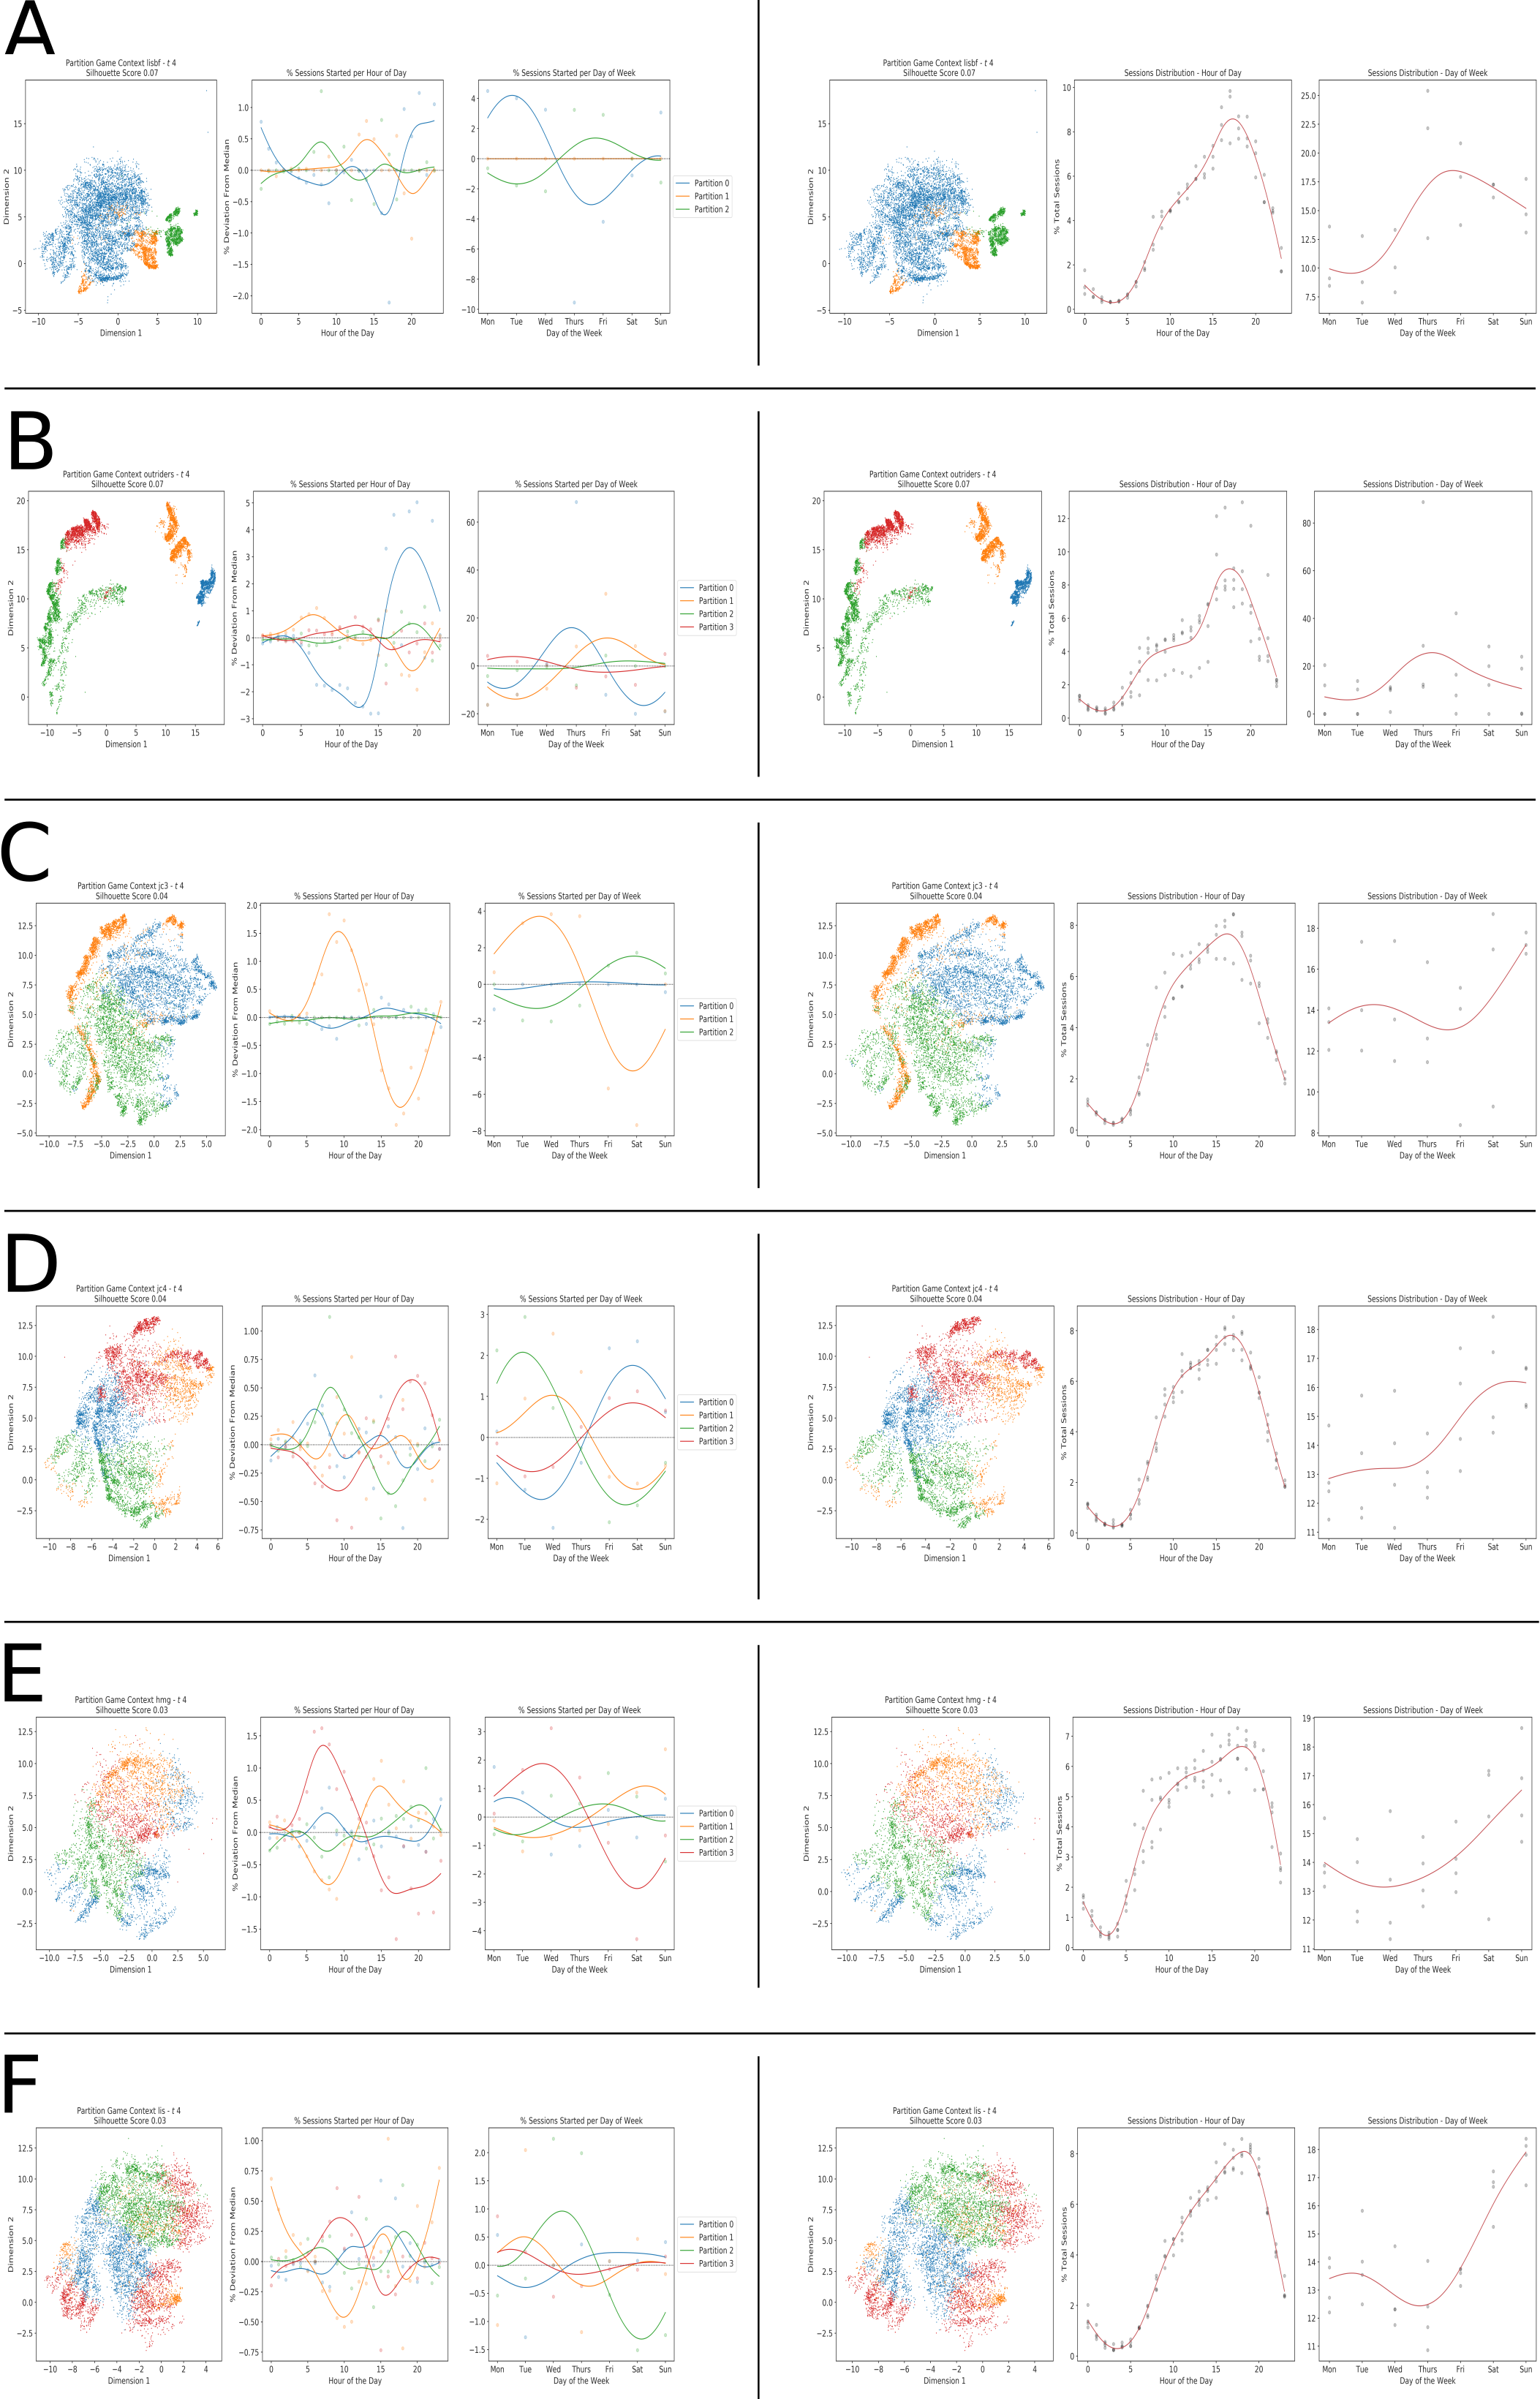
\includegraphics[width=0.7\textwidth]{images/appendix_D/clust_env_all.png}
\centering
\caption[Partitions of the representations generated by the RNN architecture and its improved versio from the environmental metrics]{The two panels show the individuated partitions and associated profiles generated by applying Mini Batch KMeans to the representation generated by the RNN architecture and its improved version. All representations have been generated from the environmental input.}
\label{partition_rnn_env} 
\end{figure}
\FloatBarrier

\section{Partitions game events metrics representations}
\label{partitions_game_events}